\documentclass{ltjsreport}

\usepackage{physics}
\usepackage{tikz}
\usepackage{here}
\usepackage{amsmath}
\usepackage{amsthm}

\usetikzlibrary{arrows}

\title{物理と微分積分}
\author{toma09to}

\renewcommand{\proofname}{\textbf{証明}}

\begin{document}

\maketitle

%\chapter{はじめに}
%
%微分積分と物理に、とても深い関わりがあるのは知っての通りだろう。
%しかし、我々が受けた授業は高校物理の教科書に従っていて、高校のカリキュラムの関係上、微分積分に関する内容に\emph{一切触れない}。
%これでは、単に数式を覚えるだけになってしまい、本質の理解とは程遠い。
%そこで、高校物理の教科書に沿って話を進めつつ、その解説により高度な数学を用いることで、より一般的な知識を得られるようにする。

\chapter{ベクトルの演算}

これからの解説において、位置や速度などの様々なベクトル量に演算を行っていくことになる。
ここでは、今後必要となる演算について解説していく。
なお、今後ベクトル量は太字(ex. $\vb{a}$)で表すこととする。

\section{ベクトルの大きさ}

あるベクトル$\vb{a}=(a_x, a_y, a_z)$を考える。
このベクトルの大きさ$|\vb{a}|$は以下のように表される。
\begin{equation}
    |\vb{a}| = \sqrt{a_x^2+a_y^2+a_z^2}
\end{equation}

なお、$\vb{a}=(a_x, a_y)$のときは以下のようになる。
\begin{equation}
    |\vb{a}| = \sqrt{a_x^2+a_y^2}
\end{equation}

これらは、ピタゴラスの定理(三平方の定理)から簡単に確認できる。

なお、大きさが1のベクトルを\emph{単位ベクトル}という。

\section{ベクトルのスカラー倍}

あるベクトル$\vb{a}$と同じ向きを持ち、長さが$k$倍のベクトルを$k\vb{a}$と表す。
ここで、$k < 0$のときベクトルの向きは逆向きになる。
\begin{figure}[H]
    \centering
    \begin{tikzpicture}
        \draw[->,>=stealth,semithick](0,0)--(0.5,1)node[right]{$\vb{a}$};
        \draw[->,>=stealth,semithick](1,0)--(2,2)node[right]{$2\vb{a}$};
        \draw[->,>=stealth,semithick](2,0)--(1,-2)node[right]{$-2\vb{a}$};
        \draw[thin](-1,0)--(3,0);
    \end{tikzpicture}
    \caption{ベクトルのスカラー倍の例}
    \label{ベクトルのスカラー倍の例}
\end{figure}

また、$\vb{a}=(a_x, a_y, a_z)$としたとき、ベクトルのスカラー倍について以下が成り立つ。
\begin{equation}
    k\vb{a} = (ka_x, ka_y, ka_z)
\end{equation}
すなわち、成分を全て$k$倍すればよい。

なお、ベクトル$\vb{a}$に対して、逆向きで同じ大きさを持つ$-\vb{a}$を\emph{逆ベクトル}と呼ぶ。

\section{ベクトルの加減算}

ある2つのベクトル$\vb{a}, \vb{b}$について、ベクトルの和$\vb{a}+\vb{b}$は図\ref{ベクトルの和}のように、$\vb{a}$の終点と$\vb{b}$の始点を重ねた時の$\vb{a}$の始点と$\vb{b}$の終点を結ぶベクトルとして定義される。
\begin{figure}[H]
    \centering
    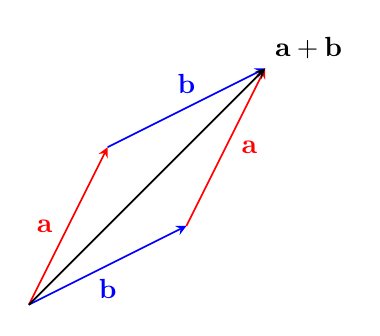
\begin{tikzpicture}
        \draw[red,->,>=stealth,semithick](0,0)--(1,2);
        \draw[blue,->,>=stealth,semithick](1,2)--(3,3);
        \draw[blue,->,>=stealth,semithick](0,0)--(2,1);
        \draw[red,->,>=stealth,semithick](2,1)--(3,3);
        \draw[->,>=stealth,semithick](0,0)--(3,3)node[above right]{$\vb{a}+\vb{b}$};
        \draw(0.2,1)node[red]{$\vb{a}$};
        \draw(2,2.8)node[blue]{$\vb{b}$};
        \draw(1,0.2)node[blue]{$\vb{b}$};
        \draw(2.8,2)node[red]{$\vb{a}$};
    \end{tikzpicture}
    \caption{ベクトルの和}
    \label{ベクトルの和}
\end{figure}

なお、この図から明らかな通り、
\begin{equation}
    \vb{a}+\vb{b} = \vb{b}+\vb{a}
\end{equation}
が成り立つ。

$\vb{a}=(a_x, a_y, a_z),\vb{b}=(b_x, b_y, b_z)$とすると、以下が成り立つ。
\begin{equation}
    \vb{a}+\vb{b} = (a_x+b_x, a_y+b_y, a_z+b_z)
\end{equation}
すなわち、対応する成分同士を足し合わせれば良い。

また、ベクトルの差$\vb{a}-\vb{b}$は、$\vb{a}+(-\vb{b})$という形で定義でき、成分で表すと、
\begin{equation}
    \vb{a}-\vb{b} = (a_x-b_x, a_y-b_y, a_z-b_z)
\end{equation}
となる。

\section{ベクトルの内積}

ベクトルの内積は、2つの方法で定義される。

2つのベクトル$\vb{a}, \vb{b}$について、$\vb{a}$と$\vb{b}$のなす角を$\theta$とおく。
\begin{figure}[H]
    \centering
    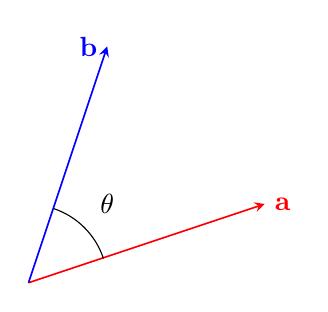
\begin{tikzpicture}
        \draw[red,->,>=stealth,semithick](0,0)--(3,1)node[right]{$\vb{a}$};
        \draw[blue,->,>=stealth,semithick](0,0)--(1,3)node[left]{$\vb{b}$};
        \draw(0.9511,0.3090)arc[start angle=18.4,end angle=71.5,radius=1];
        \draw(1,1)node{$\theta$};
    \end{tikzpicture}
    \caption{2つのベクトル}
    \label{2つのベクトル}
\end{figure}

これらの内積$\vb{a}\cdot\vb{b}$は、以下のように表される。
\begin{equation}
    \vb{a}\cdot\vb{b} = |\vb{a}||\vb{b}|\cos\theta
\end{equation}
これは、$\vb{a}$の大きさと$\vb{b}$の$\vb{a}$の方向の成分の積、または、$\vb{b}$の大きさと$\vb{a}$の$\vb{b}$の方向の成分の積を表す。

また、$\vb{a}=(a_x,a_y,a_z),\vb{b}=(b_x,b_y,b_z)$とすると、$\vb{a}\cdot\vb{b}$は以下のようにも表せる。
\begin{equation}
    \vb{a}\cdot\vb{b} = a_xb_x+a_yb_y+a_zb_z
\end{equation}

\begin{proof}
    $\vb{a}$の終点をA、$\vb{b}$の終点をB、$\vb{a}$、$\vb{b}$の始点をOとする。

    \triangle{AOB}について余弦定理を用いると、
    \begin{align}
        \cos\theta &= \frac{OA^2+OB^2-AB^2}{2OA \cdot OB} \\
                   &= \frac{|\vb{a}|^2+|\vb{b}|^2-|\vb{b}-\vb{a}|^2}{2|\vb{a}||\vb{b}|} \\
                   &= \frac{a_xb_x+a_yb_y+a_zb_z}{|\vb{a}||\vb{b}|}
    \end{align}

    したがって、
    \begin{align}
        \vb{a}\cdot\vb{b} &= |\vb{a}||\vb{b}|\cos\theta \\
                     &= |\vb{a}||\vb{b}|\frac{a_xb_x+a_yb_y+a_zb_z}{|\vb{a}||\vb{b}|} \\
                     &= a_xb_x+a_yb_y+a_zb_z
    \end{align}
\end{proof}

これら2つの定義からわかる通り、内積は可換な操作であり、
\begin{equation}
    \vb{a}\cdot\vb{b} = \vb{b}\cdot\vb{a}
\end{equation}
が成り立つ。

\section{ベクトルの外積}

ベクトルの外積とは、2つの3次元ベクトルから1つの3次元ベクトルを生成する操作である。
2つのベクトル$\vb{a},\vb{b}$の外積$\vb{a}\times\vb{b}$は、図\ref{ベクトルの外積}のようになる。
\begin{figure}[H]
    \centering
    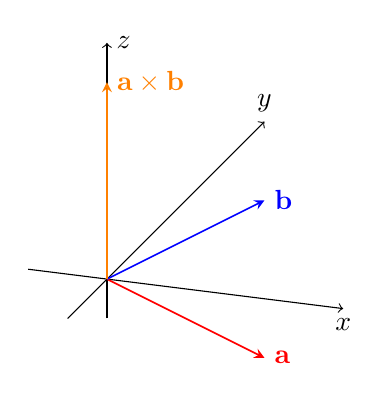
\begin{tikzpicture}
        \draw[->](-1,0.125)--(3,-0.375)node[below]{$x$};
        \draw[->](-0.5,-0.5)--(2,2)node[above]{$y$};
        \draw[->](0,-0.5)--(0,3)node[right]{$z$};
        \draw[red,->,>=stealth,semithick](0,0)--(2,-1)node[right]{$\vb{a}$};
        \draw[blue,->,>=stealth,semithick](0,0)--(2,1)node[right]{$\vb{b}$};
        \draw[orange,->,>=stealth,semithick](0,0)--(0,2.5)node[right]{$\vb{a}\times\vb{b}$};
    \end{tikzpicture}
    \caption{ベクトルの外積}
    \label{ベクトルの外積}
\end{figure}

$\vb{a}\times\vb{b}$の大きさは、$\vb{a}$と$\vb{b}$が作る平行四辺形の面積に等しく、向きは$\vb{a},\vb{b}$を含む平面に垂直である。
そのような向きは上下2通り考えられるが、$\vb{a}$から$\vb{b}$の方向に回転したときに右ねじが進む方向をとる。
また、同じベクトルの外積を考えると、平行四辺形の面積が0になることから、
\begin{equation}
    \vb{a}\times\vb{a} = \vb{0}
\end{equation}
となることがわかる。
さらに、2つのベクトルを入れ替えると、向きが逆になる。すなわち、
\begin{equation}
    \vb{b}\times\vb{a} = -\vb{a}\times\vb{b}
\end{equation}
が成り立つ。これは外積が可換な操作でないことを示している。

ベクトルの外積を成分表示すると、以下のようになる。
\begin{equation}
    \vb{a}\times\vb{b} = (a_yb_z-a_zb_y, a_zb_x-a_xb_z, a_xb_y-a_yb_x)
\end{equation}
とても奇妙な見た目をしているが、きちんと証明をすることができる。
なお、以下の証明で用いる分配則についてはあまり自明ではないが、ここでは証明されているものとするので各自調べて欲しい。

\begin{proof}
    $\vb{e_x}=(1,0,0),\vb{e_y}=(0,1,0),\vb{e_z}=(0,0,1)$とすると、
    \begin{gather}
        \vb{e_x}\times\vb{e_y}=\vb{e_z} \\
        \vb{e_y}\times\vb{e_z}=\vb{e_x} \\
        \vb{e_z}\times\vb{e_x}=\vb{e_y}
    \end{gather}
    となる。
    これは、図形的に確認することができる。

    また、
    \begin{gather}
        \vb{a} = a_x\vb{e_x}+a_y\vb{e_y}+a_z\vb{e_z} \\
        \vb{b} = b_x\vb{e_x}+b_y\vb{e_y}+b_z\vb{e_z}
    \end{gather}
    と表すことができる。

    したがって、
    \begin{align}
        \vb{a}\times\vb{b} &= (a_x\vb{e_x}+a_y\vb{e_y}+a_z\vb{e_z})\times(b_x\vb{e_x}+b_y\vb{e_y}+b_z\vb{e_z}) \\
                           &= (a_yb_z-a_zb_y)(\vb{e_y}\times\vb{e_z})+(a_zb_x-a_xb_z)(\vb{e_z}\times\vb{e_x})+(a_xb_y-a_yb_x)(\vb{e_x}\times\vb{e_y}) \\
                           &= (a_yb_z-a_zb_y,a_zb_x-a_xb_z,a_xb_y-a_yb_x)
    \end{align}
\end{proof}

\section{ベクトルのスカラー微分}

各成分が$t$に依存するようなベクトル$\vb{a}(t)=(f_x(t),f_y(t),f_z(t))$(ベクトル関数)を$t$で微分すると、結果はベクトルとなり以下のように表される。
\begin{equation}
    \frac{d\vb{a}(t)}{dt} = (\frac{d}{dt}f_x(t),\frac{d}{dt}f_y(t),\frac{d}{dt}f_z(t))
\end{equation}
すなわち各成分を微分すれば良い。

$\vb{a}(t),\vb{b}(t)$をベクトル関数、$f(t)$をスカラー関数、$\alpha$をスカラー定数とすると、以下の性質が成り立つ。

\begin{align}
    \frac{d(\alpha\vb{a}(t))}{dt}    &= \alpha\frac{d\vb{a}(t)}{dt} \\
    \frac{d(f(t)\vb{a}(t))}{dt}      &= \frac{df(t)}{dt}\vb{a}(t) + f(t)\frac{d\vb{a}(t)}{dt} \\
    \frac{d(\vb{a}\pm\vb{b})}{dt}    &= \frac{d\vb{a}}{dt}\pm\frac{d\vb{b}}{dt} \\
    \frac{d(\vb{a}\cdot\vb{b})}{dt}  &= \frac{d\vb{a}}{dt}\cdot\vb{b} + \vb{a}\cdot\frac{d\vb{b}}{dt} \\
    \frac{d(\vb{a}\times\vb{b})}{dt} &= \frac{d\vb{a}}{dt}\times\vb{b} + \vb{a}\times\frac{d\vb{b}}{dt}
\end{align}

\section{ベクトルのスカラー積分}

各成分が$t$に依存するようなベクトル$\vb{a}(t)=(f_x(t),f_y(t),f_z(t))$(ベクトル関数)を$t$で不定積分すると、結果はベクトルとなり以下のように表される。
\begin{equation}
    \int\vb{a}dt = (\int f_x(t)dt, \int f_y(t)dt, \int f_z(t)dt)
\end{equation}
$\vb{a}(t)$が導関数となるようなベクトル関数$\vb{d}(t)$を用いると以下のように表される。
ただし、$\vb{c}$はベクトル定数である。
\begin{equation}
    \int\vb{a}dt = \vb{d}(t)+\vb{c}
\end{equation}

定積分についても同様に、
\begin{equation}
    \int_a^b\vb{a}dt = (\int_a^b f_x(t)dt, \int_a^b f_y(t)dt, \int_a^b f_z(t)dt)
\end{equation}
と表すことができる。

また、$\vb{d}(t)$を$\vb{a}(t)$の不定積分の一つとすると、スカラー関数のときと同様に、
\begin{equation}
    \int_a^b\vb{a}dt = \left[ \vb{d}(t) \right]_a^b = \vb{d}(b)-\vb{d}(a)
\end{equation}
が成り立つ。

\chapter{運動の法則}

\section{位置・速度・加速度}

位置$\vb{r}$を時間微分すると速度$\vb{v}$になり、速度を時間微分すると加速度$\vb{a}$になることから、以下の関係が成り立つ。
ただし、$\vb{v_0}$は初速度、$\vb{r_0}$は初期位置を示す。
\begin{align}
    \frac{d\vb{r}}{dt} &= \vb{v} & \frac{d\vb{v}}{dt} &= \vb{a} \\
    \int\vb{a}dt &= \vb{v}+\vb{v_0} & \int\vb{v}dt &= \vb{r}+\vb{r_0}
\end{align}

\section{ニュートンの運動方程式}

前節の関係を用いると、ニュートンの運動方程式は以下のように表すことができる。
\begin{equation}
    \vb{F} = m\vb{a} = m\frac{d\vb{v}}{dt} = m\frac{d^2\vb{r}}{dt^2}
\end{equation}

\section{等速直線運動}

物体の速度が$\vb{v}=(v_x,v_y,v_z)$で一定であるとすると、時刻$t_1$から$t_2$までの間の変位$\vb{x}$は、
\begin{equation}
    \vb{x} = \int_{t_1}^{t_2}\vb{v}dt = (t_2-t_1)\vb{v} = (v_x(t_2-t_1),v_y(t_2-t_1),v_z(t_2-t_1))
\end{equation}
となる。

\section{等加速度直線運動}

物体の加速度が$\vb{a}=(a_x,a_y,a_z)$で一定であるとすると、

\end{document}
